\chapter{Generalidades}
	
	
	\section{Objetivos}\label{sec:2.1}

\subsection{Objetivo general}\label{sec:2.1.1}

Desarrollar un Sistema  Integral de Indicadores que permita medir, evaluar y controlar los procesos realizados por cada departamento en el Instituto Tecnol�gico de Tlahuac, basado en los lineamientos establecidos por la TecNM en el Sistema de Gesti�n de Calidad, para lograr realizar una gesti�n eficaz y de calidad de los mismos.\\

Lorem ipsum dolor sit amet, consectetur adipiscing elit. Proin sagittis sem non ex dapibus, tincidunt malesuada tortor posuere. Suspendisse rutrum fermentum turpis, at feugiat est cursus ac. Praesent ac gravida enim. Fusce eget eleifend nisi. Nulla facilisi. Nam porta diam nec nulla aliquam, sed mollis augue scelerisque. Sed non tempus quam. Aliquam et sem fringilla, pretium leo et, semper justo. Quisque ultrices elementum mi, ac placerat purus suscipit nec. Nulla ligula sem, tristique in vehicula non, malesuada at quam. Phasellus posuere neque ac ultricies pharetra.

\subsection{Objetivos espec\'ificos}\label{sec:2.1.2}
\begin{itemize}
    \item Eficaz an�lisis de requerimientos. 
    \item Correcta toma de datos y adecuadas entrevistas.
    \item Adecuado desarrollo del sistema.
    \item Implementaci�n oportuna de pruebas de funcionamiento.
    \item Implemetaci�n de pruebas en ambiente y de producci�n.
\end{itemize}

\section{Justificaci\'on}\label{sec:2.2}
\paragraph{}%parrafo 1
Lorem ipsum dolor sit amet, consectetur adipiscing elit. Proin sagittis sem non ex dapibus, tincidunt malesuada tortor posuere. Suspendisse rutrum fermentum turpis, at feugiat est cursus ac. Praesent ac gravida enim. Fusce eget eleifend nisi. Nulla facilisi. Nam porta diam nec nulla aliquam, sed mollis augue scelerisque. Sed non tempus quam. Aliquam et sem fringilla, pretium leo et, semper justo. Quisque ultrices elementum mi, ac placerat purus suscipit nec. Nulla ligula sem, tristique in vehicula non, malesuada at quam. Phasellus posuere neque ac ultricies pharetra.
\paragraph{}%parrafo 2
Lorem ipsum dolor sit amet, consectetur adipiscing elit. Proin sagittis sem non ex dapibus, tincidunt malesuada tortor posuere. Suspendisse rutrum fermentum turpis, at feugiat est cursus ac. Praesent ac gravida enim. Fusce eget eleifend nisi. Nulla facilisi. Nam porta diam nec nulla aliquam, sed mollis augue scelerisque. Sed non tempus quam. Aliquam et sem fringilla, pretium leo et, semper justo. Quisque ultrices elementum mi, ac placerat purus suscipit nec. Nulla ligula sem, tristique in vehicula non, malesuada at quam. Phasellus posuere neque ac ultricies pharetra.

\section{Caracterizaci\'on de la empresa en la que particip\'o}\label{sec:2.3}

\subsection{Datos generales de la empresa}\label{sec:2.3.1}
\begin{itemize}
         \item \textbf{Empresa:} 
         \item \textbf{Direcci�n:} 
         \vspace*{1in}
         \begin{figure}[htb]
            \centering
            %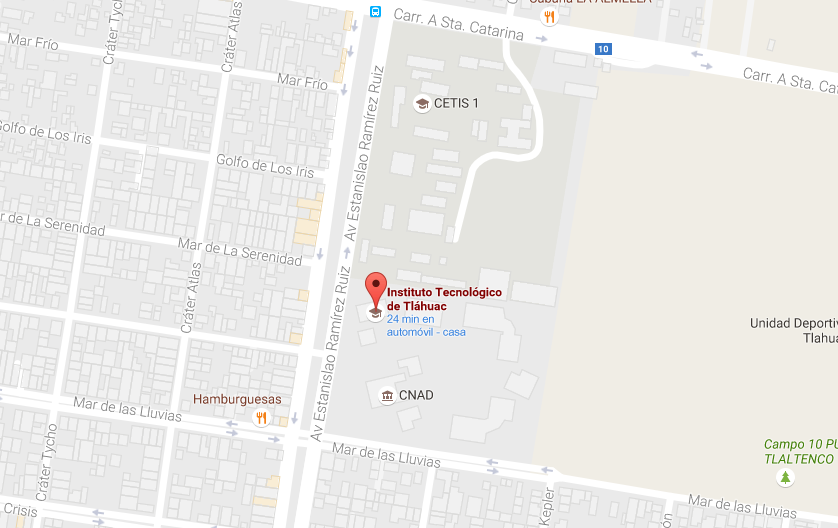
\includegraphics{croquis}
            \caption{Croquis de ubicaci�n.} \label{fig:croquis}
         \end{figure}
         \item \textbf{Tel�fono:} 
         \item \textbf{Direcci�n de correo electr�nico:} 
         \item Giro, misi�n, visi�n valores y pol�ticas de calidad:
         \item \textbf{Estructura organizacional:}
    \end{itemize}

\subsection{Descripci\'on del departamento o  \'area de trabajo}\label{sec:2.3.2}
\begin{itemize}
         \item \textbf{Nombre del departamento:} 
         \item \textbf{Estructura departamental:} 
         \item \textbf{Descripci�n del  �rea en que se particip�:} 
    \end{itemize}

\section{Problemas a resolver (prioriz\'andolos)}\label{sec:2.4}
\paragraph{}
Lorem ipsum dolor sit amet, consectetur adipiscing elit. Proin sagittis sem non ex dapibus, tincidunt malesuada tortor posuere. Suspendisse rutrum fermentum turpis, at feugiat est cursus ac. Praesent ac gravida enim. Fusce eget eleifend nisi. Nulla facilisi. Nam porta diam nec nulla aliquam, sed mollis augue scelerisque. Sed non tempus quam. Aliquam et sem fringilla, pretium leo et, semper justo. Quisque ultrices elementum mi, ac placerat purus suscipit nec. Nulla ligula sem, tristique in vehicula non, malesuada at quam. Phasellus posuere neque ac ultricies pharetra.
\vspace*{0.6in}

\section{Alcances y limitaciones}\label{sec:2.5}
\textbf{Alcances}
\begin{itemize}
         \item 
         \item 
         \item 
         \item
    \end{itemize}
    
\textbf{Limitaciones}
\begin{itemize}
         \item 
         \item
         \item 
         \item
    \end{itemize}
